\documentclass{article}
%==============================================================================%
%	                          Packages                                     %
%==============================================================================%
% Packages
\usepackage[utf8]{inputenc}
\usepackage{graphicx}
\usepackage{amsmath}
\usepackage{amssymb}
\usepackage{braket}
\usepackage[margin=0.7in]{geometry}
\usepackage[version=4]{mhchem}
\usepackage{float}
%==============================================================================%
%                           User-Defined Commands                              %
%==============================================================================%
% User-Defined Commands
\newcommand{\be}{\begin{equation}}
\newcommand{\ee}{\end{equation}}
\newcommand{\benum}{\begin{enumerate}}
\newcommand{\eenum}{\end{enumerate}}
\newcommand{\pd}{\partial}
\newcommand{\dg}{\dagger}
%==============================================================================%
%                             Title Information                                %
%==============================================================================%
\title{Chem237: Lecture 5}
\date{4/11/18}
\author{Shane Flynn,Moises Romero}
%==============================================================================%
%	Everyone Please Make Comments if Something Needs to be Reviewed        %
%                           Or just fix it yourself!                           %
%==============================================================================%
\begin{document}
\maketitle
\section*{Integrals Continued}
%==============================================================================%
\section*{Complex Calculus }
Complex Calculus is a large field (typically a 1-year course) we will highlight some useful integration techniques using the complex plane. 

\subsection*{Analytic Function}
Consider the 2D complex plane. 
%==============================================================================%
%%%%%%%%%%%%%%%%%%%%%%%%%%%%%%%%%%%%%%%%%%%%%%%%%%%%%%%%%%%%%%%%%%%%%%%%%%%%%%%%
% We need a 'professional' version of this figure
%%%%%%%%%%%%%%%%%%%%%%%%%%%%%%%%%%%%%%%%%%%%%%%%%%%%%%%%%%%%%%%%%%%%%%%%%%%%%%%%
%==============================================================================%
\begin{figure}[h]
  \centering
  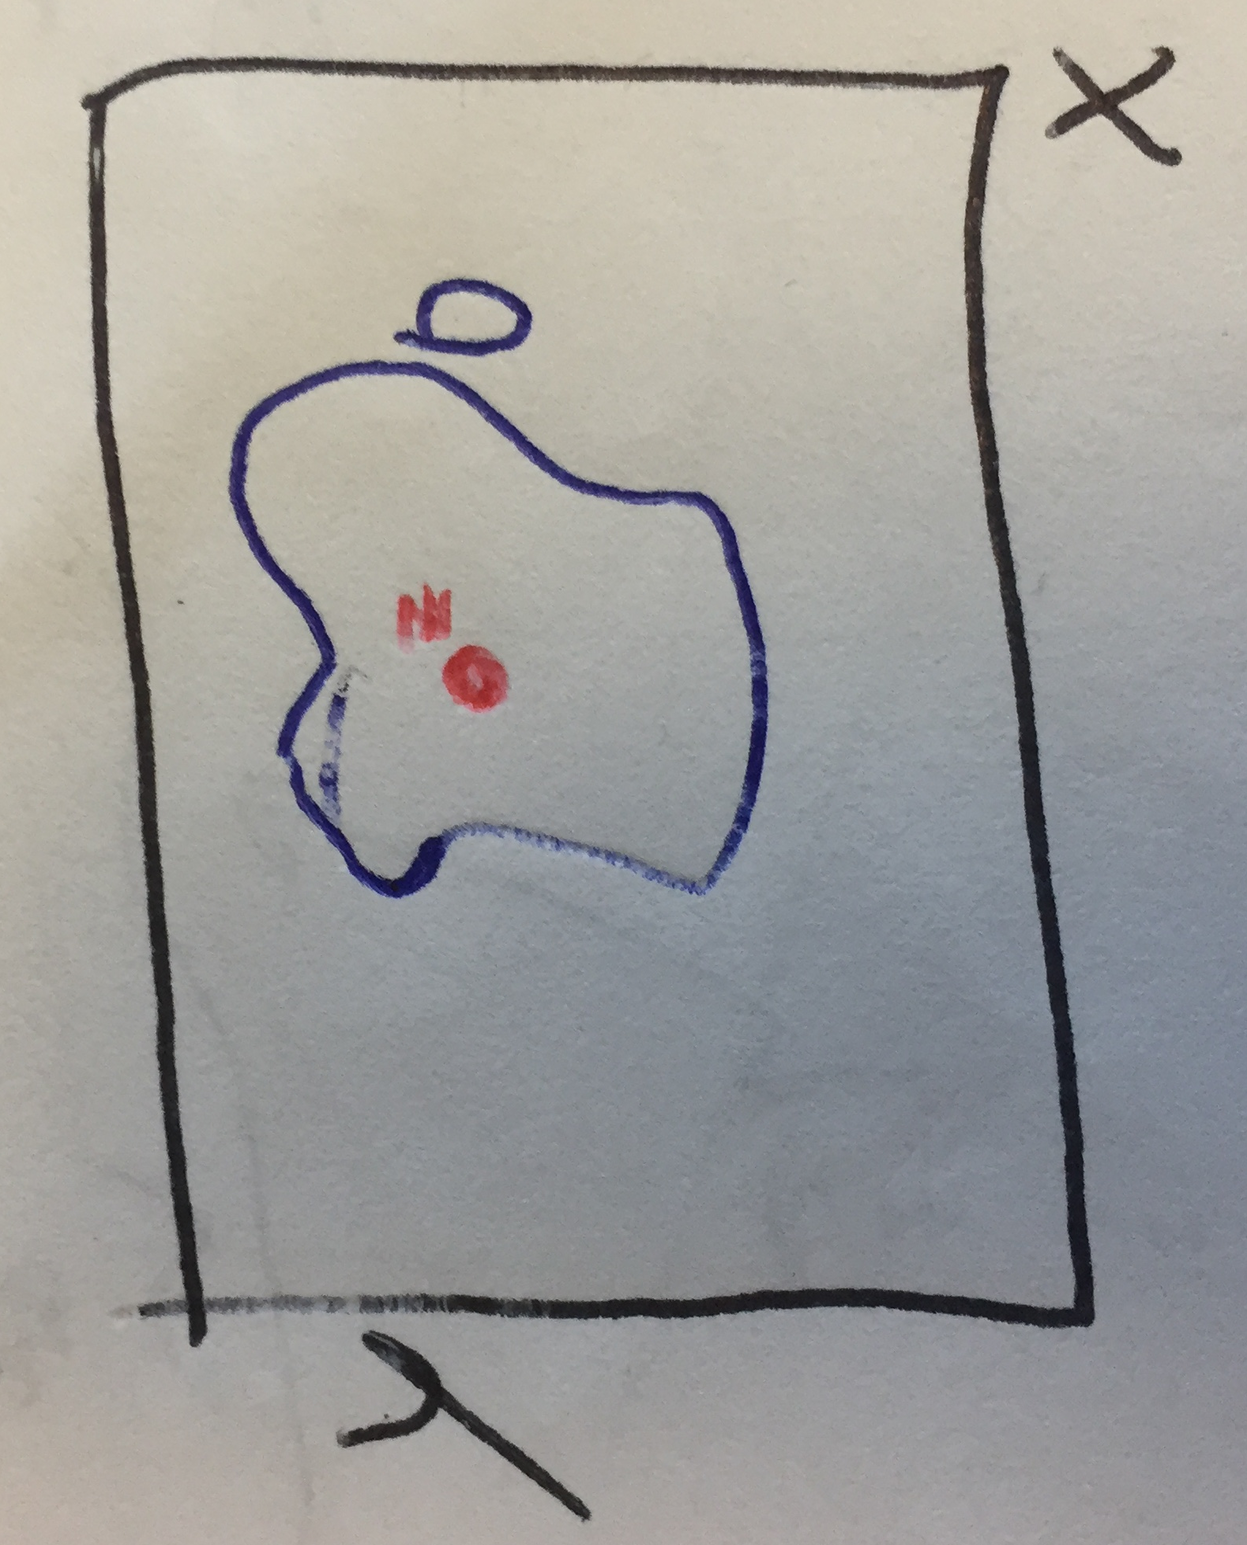
\includegraphics[scale=0.2]{Figures/complex.png}
    \caption{Under-Damped HO. The real part of the solution (blue), for the un-driven, under-damped harmonic oscillator.
    The dotted line (green) shows that the amplitude of the function (and the the function itself) slowly decays to zero over time.}
  \label{fig:under_damped}
\end{figure}
Analytic function in domain (D) if it has derivative for any Z in D.
\be
f'(z) = \lim_{h\to 0} \frac{f(z+h)-f(z)}{h}
\ee
f(z) is regular in D if it is analytic and single valued in D.
Examples of non singled valued functions are square roots
$f(z) = \sqrt{z}$ and logarithm functions $f(z)=\ln{(1+z)}$
\subsection*{Cauchy Riemann equations}
The Cauchy-Riemann equations are used to check if a complex function is analytic (sometimes referred to as holomorphic), in other words if it is differentiable.
It is often useful to define complex functions into their real and complex parts as follows :
\be
f(z) = u(x,y) + iv(x,y)
\ee
The Cauchy-Riemann equations are derived from taking a  differential with respect to x and y  and then relating the Real part and imaginary part. Note: that for the imaginary piece we multiply by i thus getting a negative:
\be
\begin{split}
\frac{\partial f}{\partial x} = \frac{\partial u}{\partial x}+ i\frac{\partial v}{\partial x} &= \frac{1}{i}\frac{\partial f}{\partial y} = \frac{1}{i}\frac{\partial u}{\partial y}+\frac{\partial v}{\partial x} \\
\frac{\partial u}{\partial x} &= \frac{\partial v}{\partial y} \\
\frac{\partial v}{\partial x} &= - \frac{\partial u}{\partial y}
\end{split}
\ee
Example of an analytic function :
\be
\begin{split}
 f(z)=z^2 &= x^2 - y^2 + i(2xy) \\
 u &= x^2+y^2\\
 v &=2xy \\
 \frac{\partial u}{\partial x} &= 2x \frac{\partial v}{\partial y}\\
\frac{\partial v}{\partial x} &=2y - \frac{\partial u}{\partial y}
\end{split}
\ee
Example of a non-analytic :
\be
\begin{split}
    f=z*=x-iy  \\
\frac{\partial u}{\partial x} = 1 \neq \frac{\partial v}{\partial y} = -1
\end{split}
\ee
\subsection*{Cauchy-Theorem}
The Cauchy theorem states an integral is path independent if f(z) is regular in D $\epsilon$ L. Where L denotes a path integral.
\be
\left \int\limits_L\right_{z_1}^{z_2} f(z) dz
\ee
More commonly it is written as a contour:
\be
\oint\limits_{C \epsilon D} f(z) dz = 0
\ee

The definition of an analytic function is only the first derivative of f(z) exists.
If f(z) is ? in D :
\be
\frac{d^n}{dz^n} f(z)
\ee
exists for any n. $f^(n)(z)$ is a result function in D.


\subsection*{Cauchy Integral Formula}
The general formula for the Cauchy integral formula is as follows :
\be
f^{n}(z) = \frac{d^n f}{dz^n}  \frac{n!}{2\pi i } \oint \frac{f(w) dw}{(w-z)^{n+1}}
\ee
Where n is the order of your function.
%==============================================================================%
%	These all require proofs as well as many of the
% contour graphs that vlad drew out in class.    %
%                                                     %
%==============================================================================%














\end{document}
